\documentclass[12pt,letterpaper]{article}

\usepackage{amsmath, amsthm, amsfonts, amssymb}
\usepackage{microtype, parskip, graphicx}
\usepackage[comma,numbers,sort&compress]{natbib}
\usepackage{lineno}
\usepackage{longtable}
\usepackage{docmute}
\usepackage{caption, subcaption, multirow, morefloats, rotating}
\usepackage{wrapfig}
\usepackage{hyperref}

\frenchspacing

\begin{document}
\section*{Materials and Methods}

\subsection*{Taxon occurrences and species-level information}
All fossil occurrence information used in this analysis was downloaded from the Paleobiology Database (PBDB). The initial download restricted all occurrences to all Mammalia observed in North America between the Maastrichtian (XX Mya) and Gelasian (XX Mya) stages. Occurrences were then further limited to those occurring between 64 and 2 million years ago (Mya). Taxonomic, stratigraphic, and ecological metadata for each occurrence and spcies was also downloaded. A new download for a raw, unfiltered PBDB datafile following the same criterion used here is available at \url{http://goo.gl/2slgeU}. The raw datafiles used as a part of this study, along with all code for filtering and manipulating this download is available at GITHUB.
%https://paleobiodb.org/data1.2/occs/list.csv?datainfo&rowcount&base_name=Mammalia&taxon_reso=species&interval=Maastrichtian,Gelasian&cc=NOA&show=class,genus,ecospace,loc,strat,stratext,lith,acconly. 

After download, the raw occurrence data was then sorted, cleaned, and manipulated programmatically before analysis. Many species taxonomic assignments as present in the raw PBDB data were updated for accuracy and consistency. For example, species classified in the order Artidodactyla were reclassified as Cetartiodactyla. These re-assignments follow \citet{Smits2015b} which were based on taxonomies present in the Encylopedia of Life WEBSITE and \citet{Janis1998,Janis2008}. All taxa who's life habit was classified as either volant (i.e. Chiroptera) or aquatic (e.g. Cetacea) were excluded from this analysis because of both differences in fossilization potential and environmental context as well as their lack of direct applicability to the study of terrestrial species pools.

Species ecotype is defined here as the interaction between life habit and diet categories, the goal of which is to classify species based on the manner with which they interact with their environment. Most mammal species records in the PBDB have life habit and dietary category assignments. In order to simplify interpretation, analysis, and per ecotype sample size these classifications were coarsened in a similar manner to \citep{Smits2015b} following Table \ref{tab:trait_cats}. Additionally for this study, the life history category was further broken up to better reflect the diversity of mammal locomotor modes. Ground dwelling species locomotor categories were reassigned based on their ankle posture associated with their taxonomic group as described in Table \ref{tab:posture} \citep{Carrano1999}. Ecotype categories with less than 10 total species of that combination were excluded, yielding a total of 18 observed ecotypes out of a possible 24.

\begin{table}[ht]
  \centering
  \caption{Species trait assignments in this study are a coarser version of the information available in the PBDB. Information was coarsened to improve per category sample size and uniformity and followed this table.}
  \begin{tabular}[ht]{ l | l | l }
    \hline
    \multicolumn{2}{ c |}{This study} & PBDB categories \\
    \hline \hline
    \multirow{4}{*}{Diet} & Carnivore & Carnivore \\
    & Herbivore & Browser, folivore, granivore, grazer, herbivore. \\
    & Insectivore & Insectivore. \\
    & Omnivore & Frugivore, omnivore. \\ 
    \hline
    \multirow{3}{*}{Locomotor} & Arboreal & Arboreal.\\
    & Ground dwelling & Fossorial, ground dwelling, semifossorial, saltatorial. \\
    & Scansorial & Scansorial. \\
    \hline
  \end{tabular}
  \label{tab:trait_cats}
\end{table}


\begin{center}
  \begin{longtable}{ l l l }
    \caption[Posture assignment based on taxonomy]{Posture assignment based on taxonomy} \label{tab:posture} \\

    Order & Family & Stance \\ \hline
    \endfirsthead
  
    \multicolumn{3}{p{\textwidth}}{{ \bfseries \tablename\ \thetable{} -- continued from previous page}} \\
    \hline Order & Family & Stance \\ \hline
    \endhead
      
    \hline \multicolumn{3}{p{\textwidth}}{{Continued on next page}} \\ \hline
    \endfoot
  
    \hline \hline
    \endlastfoot
  
    & Ailuridae & plantigrade \\ 
    & Allomyidae & plantigrade \\ 
    & Amphicyonidae & plantigrade \\ 
    & Amphilemuridae & plantigrade \\ 
    & Anthracotheriidae & digitigrade \\ 
    & Antilocapridae & unguligrade \\ 
    & Apheliscidae & plantigrade \\ 
    & Aplodontidae & plantigrade \\ 
    & Apternodontidae & scansorial \\ 
    & Arctocyonidae & unguligrade \\ 
    & Barbourofelidae & digitigrade \\ 
    & Barylambdidae & plantigrade \\ 
    & Bovidae & unguligrade \\ 
    & Camelidae & unguligrade \\ 
    & Canidae & digitigrade \\ 
    & Cervidae & unguligrade \\ 
    & Cimolodontidae & scansorial \\ 
    & Coryphodontidae & plantigrade \\ 
    & Cricetidae & plantigrade \\ 
    & Cylindrodontidae & plantigrade \\ 
    & Cyriacotheriidae & plantigrade \\ 
    & Dichobunidae & unguligrade \\ 
    Dinocerata &  & unguligrade \\ 
    & Dipodidae & digitigrade \\ 
    & Elephantidae & digitigrade \\ 
    & Entelodontidae & unguligrade \\ 
    & Eomyidae & plantigrade \\ 
    & Erethizontidae & plantigrade \\ 
    & Erinaceidae & plantigrade \\ 
    & Esthonychidae & plantigrade \\ 
    & Eutypomyidae & plantigrade \\ 
    & Felidae & digitigrade \\ 
    & Florentiamyidae & plantigrade \\ 
    & Gelocidae & unguligrade \\ 
    & Geolabididae & plantigrade \\ 
    & Glyptodontidae & plantigrade \\ 
    & Gomphotheriidae & unguligrade \\ 
    & Hapalodectidae & plantigrade \\ 
    & Heteromyidae & digitigrade \\ 
    & Hyaenidae & digitigrade \\ 
    & Hyaenodontidae & digitigrade \\ 
    & Hypertragulidae & unguligrade \\ 
    & Ischyromyidae & plantigrade \\ 
    & Jimomyidae & plantigrade \\ 
    Lagomorpha &  & digitigrade \\ 
    & Leptictidae & plantigrade \\ 
    & Leptochoeridae & unguligrade \\ 
    & Leptomerycidae & unguligrade \\ 
    & Mammutidae & unguligrade \\ 
    & Megalonychidae & plantigrade \\ 
    & Megatheriidae & plantigrade \\ 
    & Mephitidae & plantigrade \\ 
    & Merycoidodontidae & digitigrade \\ 
    Mesonychia &  & unguligrade \\ 
    & Mesonychidae & digitigrade \\ 
    & Micropternodontidae & plantigrade \\ 
    & Mixodectidae & plantigrade \\ 
    & Moschidae & unguligrade \\ 
    & Muridae & plantigrade \\ 
    & Mustelidae & plantigrade \\ 
    & Mylagaulidae & fossorial \\ 
    & Mylodontidae & plantigrade \\ 
    & Nimravidae & digitigrade \\ 
    & Nothrotheriidae & plantigrade \\ 
    Notoungulata &  & unguligrade \\ 
    & Oromerycidae & unguligrade \\ 
    & Oxyaenidae & digitigrade \\ 
    & Palaeomerycidae & unguligrade \\ 
    & Palaeoryctidae & plantigrade \\ 
    & Pampatheriidae & plantigrade \\ 
    & Pantolambdidae & plantigrade \\ 
    & Periptychidae & digitigrade \\ 
    Perissodactyla &  & unguligrade \\ 
    & Phenacodontidae & unguligrade \\ 
    Primates &  & plantigrade \\ 
    & Procyonidae & plantigrade \\ 
    & Proscalopidae & plantigrade \\ 
    & Protoceratidae & unguligrade \\ 
    & Reithroparamyidae & plantigrade \\ 
    & Sciuravidae & plantigrade \\ 
    & Sciuridae & plantigrade \\ 
    & Simimyidae & plantigrade \\ 
    & Soricidae & plantigrade \\ 
    & Suidae & digitigrade \\ 
    & Talpidae & fossorial \\ 
    & Tayassuidae & unguligrade \\ 
    & Tenrecidae & plantigrade \\ 
    & Titanoideidae & plantigrade \\ 
    & Ursidae & plantigrade \\ 
    & Viverravidae & plantigrade \\ 
    & Zapodidae & plantigrade \\ 
    \hline
  \end{longtable}
\end{center}


Estimates of species mass used as a covariate in this study were sourced from multiple databases and papers, especially those focusing on similar macroevolutionary or macrecological questions \citep{Tomiya2013,Brook2004a,Freudenthal2013,McKenna2011,Raia2012f,Smith2004}; this is similar to what was done in \citet{Smits2015b}. When species mass was not avaliable, proxy measures were used and then transformed into estimates of mass. For example, given a measurement of a mammal tooth size, it is possible and routine to estimate its mass given some regression equation. The PBDB has one or more body part measures for many species. These were used as body size proxies for many species, as was the case in \citet{Smits2015b}. Mass was log-transformed and then mean-centered and rescaled by dividing by two-times its standard deviation; this insures that the magnitude of effects for both continuous and discrete covariates are directly comparable \citep{Gelman2007,Gelman2008}.

\begin{table}[ht]
  \centering
  \caption{Regression equations used in this study for estimating body size. Equations are presented with reference to taxonomic grouping, part name, and reference.}
  \begin{tabular}{l | l | l | l}
    Group & Equation & log(Measurement) & Source \\
    \hline
    General & \(\log(m) = 1.827x + 1.81\) & lower m1 area &  \cite{Legendre1986} \\
    General & \(\log(m) = 2.9677x - 5.6712\) & mandible length & \cite{Foster2009a} \\
    General & \(\log(m) = 3.68x - 3.83\) & skull length & \cite{Luo2001} \\
    Carnivores & \(\log(m) = 2.97x + 1.681\) & lower m1 length & \cite{VanValkenburgh1990} \\
    Insectivores & \(\log(m) = 1.628x + 1.726\) & lower m1 area & \cite{Bloch1998} \\
    Insectivores & \(\log(m) = 1.714x + 0.886\) & upper M1 area & \cite{Bloch1998} \\
    Lagomorph & \(\log(m) = 2.671x - 2.671\) & lower toothrow area & \cite{Tomiya2013} \\
    Lagomorph & \(\log(m) = 4.468x - 3.002\) & lower m1 length & \cite{Tomiya2013} \\
    Marsupials & \(\log(m) = 3.284x + 1.83\) & upper M1 length & \cite{Gordon2003} \\
    Marsupials & \(\log(m) = 1.733x + 1.571\) & upper M1 area & \cite{Gordon2003} \\
    Rodentia & \(\log(m) = 1.767x + 2.172\) & lower m1 area & \cite{Legendre1986} \\
    Ungulates & \(\log(m) = 1.516x + 3.757\) & lower m1 area & \cite{Mendoza2006} \\
    Ungulates & \(\log(m) = 3.076x + 2.366\) & lower m2 length & \cite{Mendoza2006} \\
    Ungulates & \(\log(m) = 1.518x + 2.792\) & lower m2 area & \cite{Mendoza2006} \\
    Ungulates & \(\log(m) = 3.113x - 1.374\) & lower toothrow length & \cite{Mendoza2006} \\
    \hline
  \end{tabular}
  \label{tab:mass_est}
\end{table}


All fossil occurrences from 64 to 2 million years long (Mya) were binned into 31 2 million year (My) bins. This temporal length was chosen because it is approximately the resolution of the North American mammal fossil record \citep{Alroy1996a,Alroy2000g,Marcot2014}.



\subsection*{Environmental and temporal covariates}
The environmental covariates used in this study are collectively referred to as group-level covariates because they predict the response of a ``group'' of individual-level observations (i.e. species occurrences of an ecotype). Additionally, these covariates are defined for temporal bins and not the species themselves; as such they predict the parts of each species occurrence history. The group-level covariates in this study are two global temperature estimates and the Cenozoic ``plant phases'' defined by Graham CITATION. Global temperature across most of the Cenozoic was calculated from Mg/Ca isotope record from deep sea carbonates \citep{Cramer2011}. Mg/Ca based temperature estimates are preferable to the frequently used \(\delta^{18}\)O temperature proxy \citep{Zachos2001,Zachos2008,Alroy2000g,Figueirido2012} because Mg/Ca estimates do not conflate temperature with ice sheet volume and depth/stratification changes. The former is particularly important to this analysis as the current polar ice-caps appeared and grew over the Cenozoic. These properties make Mg/Ca based temperature estimates preferable for macroevolutionary and macroecological studies \citep{Ezard2016a}. Two aspects of the Mg/Ca-based temperature curve were included in this analysis: mean and range. Both were calculated as the mean of all respective estimates for each 2 My temporal bins. Both mean and range were then rescaled by subtracting the mean and then dividing by twice the standard deviation. 

The second set of environmental factors included in this study are the Cenozoic plant phases defined in Graham CITATION. Graham's plant phases are holistic descriptors of the taxonomic composition of 12 ecosystem types, which plants are present at a given time, and the relative modernity of those plant groups with younger phases representing increasingly modern taxa CITATION. Graham CITATION defines four intervals from the Cretaceous to the Pliocene, though only three of these intervals are included in this analysis. Graham's plant phases CITATION was included as a series of ``dummy variables'' encoding the three phases included in this analysis. This means that the first phase is synonymous with the intercept and subsequent phases are defined by their differences from the first phase.


\subsection*{Modelling species occurrence}
Two different models were used in this study: a pure-presence model and a birth-death model. Both models at their core are a hidden Markov model where the latent process has an absorbing state \citep{Allen2011}. The difference between these two models is if the probabilities of a species originating or surviving are considered equal or different (Table \ref{tab:transition}). Something that is important to realize is that while there are only two state ``codes'' in a presence-absence matrix (i.e. 0/1), there are in fact three states in a birth-death model: not having originated (yet), extant, and extinct. The last of these is the absorbing state, as once a species has gone extinct it cannot re-originate \citep{Allen2011}; this is made obvious in the transition matrices as the probability of an extinct species changing states is 0 (Table \ref{tab:transition}). See below for parameter explainations (Tables \ref{tab:pres_param}, and \ref{tab:bd_param}).

\begin{table}
  \begin{subtable}[t]{0.45\linewidth}
    \begin{tabular}[c]{ c c | c | c | c | }
      \cline{3-5} 
      & & \multicolumn{3}{ c |}{ State at \(t + 1\)} \\ \cline{3-5}
      & & \(0_{never}\) & 1 & \(0_{extinct}\) \\ \hline
      \multicolumn{1}{| c |}{\multirow{3}{*}{State at \(t\)}}
      & \(0_{never}\) & \(1 - \theta\)  & \(\theta\) & 0 \\ \cline{2-5}
      \multicolumn{1}{| c |}{} & 1 & 0 & \(\theta\) & \(1 - \theta\) \\ \cline{2-5}
      \multicolumn{1}{| c |}{} & \(0_{extinct}\) & 0 & 0 & 1 \\
      \hline
    \end{tabular}
    \caption{Pure-presence}
    \label{tab:pp}
  \end{subtable}
  \begin{subtable}[t]{0.45\linewidth}
    \begin{tabular}[c]{ c c | c | c | c | }
      \cline{3-5} 
      & & \multicolumn{3}{ c |}{ State at \(t + 1\)} \\ \cline{3-5}
      & & \(0_{never}\) & 1 & \(0_{extinct}\) \\ \hline
      \multicolumn{1}{| c |}{\multirow{3}{*}{State at \(t\)}}
      & \(0_{never}\) & \(1 - \phi\)  & \(\phi\) & 0 \\ \cline{2-5}
      \multicolumn{1}{| c |}{} & 1 & 0 & \(\pi\) & \(1 - \pi\) \\ \cline{2-5}
      \multicolumn{1}{| c |}{} & \(0_{extinct}\) & 0 & 0 & 1 \\
      \hline
    \end{tabular}
    \caption{Birth-death}
    \label{tab:bd}
  \end{subtable}
  \caption{Transition matrices for the pure-presence (\ref{tab:pp}) and birth-death (\ref{tab:bd}) models. Both of these models share the core machinery of discrete-time birth-death processes but make distinct assumptions about the equality of orginating and surviving (Eq. \ref{eq:pure_presence}, and \ref{eq:birth_death}). Note also that while there are only two state ``codes'' (0, 1), there are in fact three states: never having originated \(0_{never}\), present 1, extinct \(0_{extinct}\) \citep{Allen2011}.}
  \label{tab:transition}
\end{table}


\subsubsection*{Data augmentation}
All empirical presence/absence observations are potentially incomplete or observed with error. The hidden Markov model at the core of this analysis allows for observed absences to be used meaningfully to estimate the number of unobserved species. Of concern in this analysis is the unknown ``true'' size of the dataset; how many species could have actually been observed? While many species have been observed, the natural incompleteness of all observations, especially in the case of paleontological data, there are obviously many species which were never sampled \citep{Royle2008,Royle2007a}.

Let \(N\) by the total number of observed species, \(M\) be the upper limit of possible species that could have existed given some model of species occurrence, and \(N^{\ast}\) is the number of all-zero histories added to the presence absence matrix \(y\) where \(N^{\ast} = M - N\). This approach assumes that \(\hat{N} \sim \text{Binomial}(M, \psi)\) where \(\hat{N}\) is the estimated ``true'' number of species and \(\psi\) is the probability that any augmented species should actually be ``present.'' Because \(M\) is user defined, this approach effectively gives \(\psi\) a uniform prior over \(N\) to \(M\) \citep{Royle2008}. For this study, \(M = \lfloor{1.25 \times N\rfloor}\).

Data imputation is the process of estimating missing data for partially observed covariates given the other fully-observed observations and some model \citep{Gelman2007,Rubin1996}, this is simple in a Bayesian context because data are also parameters \citep{Gelman2013d}. Augmented species are fully imputed species and thus have no known mass so a mass estimate must be imputed for each possible species \citep{Royle2012b}. Assuming that mass values for augmented species are from the same distribution as observed species, the distribution of observed mass values are estimated as part of the model and new mass values are then generated from this distribution. This approach is an example of imputing covariate information that is missing completely at random \citep{Gelman2007,Royle2012b}. Because log mass values are rescaled as a part of this study, the body mass distribution is already known (\(\mathcal{N}(0, 0.5)\)) the body mass of the augmented species are generated by simple random draws from this distribution. In addition to body mass information, the augmented species need an ecotype classification. Because these species are completely unknown, they were all classified as ``augmented'' to indicate their unknown biology. This classification has no biological interpretation.



\subsubsection*{Observation process}
The type of hidden Markov model used in this study has three characteristic probabilities: probability \(p\) of observing a species given that it is present, probability \(\phi\) of a species surviving from one time to another, and probability \(\pi\) of a species first appearing \citep{Royle2008}. In this formulation, the probability of a species going extinct is \(1 - \pi\). For the pure-presence model \(\phi = \pi\), while for the birth-death model \(\phi \neq \pi\).

\begin{table}
  \centering
  \caption{Observation parameters}
  \begin{tabular}{c l l}
    Parameter & dimensions & explanation \\
    \hline
    \(y\) & \(N \times T\) & observed species presence/absence \\
    \(z\) & \(N \times T\) & ``true'' species presence/absence \\
    \(p\) & \(T\) & probability of observing a species that is present at time \(t\) \\
    \(m\) & \(N\) & species log mass, rescaled \\
    \(\alpha_{0}\) & 1 & average log-odds of \(p\) \\ % when mass = 0
    \(\alpha_{1}\) & 1 & change in average log-odds of \(p\) per change mass \\
    \(r\) & \(T\) & difference from \(\alpha_{0}\) associated with time \(t\) \\
    \(\sigma\) & 1 & standard deviation of \(r\) \\
  \end{tabular}
  \label{tab:obs_param}
\end{table}

The probability of observing a species that is present \(p\) is modeled as a logistic regression was a time-varying intercept and species mass as a covariate. The effect of species mass on \(p\) was assumed linear and constant over time and given a prior reflecting a possible positive relationship; these assumptions are reflected in the structure of the model Equation \ref{eq:obs_model}, presented here:
\begin{equation}
  \begin{aligned}
    y_{i, t} &\sim \text{Bernoulli}(p_{i, t} z_{i, t}) \\
    p_{i, t} &= \text{logit}^{-1}(\alpha_{0} + \alpha_{1} m_{i} + r_{t}) \\ 
    r_{t} &\sim \mathcal{N}(0, \sigma). \\
  \end{aligned}
  \label{eq:obs_model}
\end{equation}
The parameters associated with Equation \ref{eq:obs_model} are described in Table \ref{tab:obs_param}.


\subsubsection*{Pure-presence process}
For the pure-presence model there is only a single probability dealing with the presence of a species \(\theta\) (Table \ref{tab:pp}). This probability was modeled as multi-level logistic regression with both species-level and group-level covariates \citep{Gelman2007,Gelman2013d}. The parameters associated with pure-presence model are presented in Table \ref{tab:pres_param} and the full sampling statement in Equation \ref{eq:pure_presence}.

\begin{table}
  \centering
  \caption{Parameters for the model of presence in the pure-presence model}
  \begin{tabular}{c l l}
    Parameter & dimensions & explanation \\
    \hline
    \(z\) & \(N \times T\) & ``true'' species presence/absence \\
    \(\theta\) & \(N \times T - 1\) & probability of \(z = 1\) \\
    \(a\) & \(T - 1 \times D\) & ecotype-varying intercept; mean value of log-odds of \(\theta\) \\
    \(m\) & \(N\) & species log mass, rescaled \\
    \(b_{1}\) & 1 & effect of species mass on log-odds of \(\theta\) \\
    \(b_{2}\) & 1 & effect of species mass, squared, on log-odds of \(\theta\) \\
    \(U\) & \(T \times D\) & matrix of group-level covariates \\
    \(\gamma\) & \(U \times D\) & matrix of group-level regression coefficients \\
    \(\Sigma\) & \(D \times D\) & covariance matrix of \(a\) \\
    \(\Omega\) & \(D \times D\) & correlation matrix of \(a\) \\
    \(\tau\) & \(D\) & vector of standard deviations for each ecotype \(a_{d}\) \\
  \end{tabular}
  \label{tab:pres_param}
\end{table}

The species-level of the model (Eq. \ref{eq:pure_presence}) is a logistic regression where the intercept varies by ecotype. Additionally, species mass was included as a covariate associated with two regression coefficients allowing a quadratic relationship with log-odds of occurrence. This assumption is based on the known distribution of mammal body masses where species with intermediate mass values are more common than either small or large bodied species. These assumptions are also reflected in the choice of priors for these regression coefficients.

The values of each ecotype's intercept are themselves modeled as regressions using the group-level covariates associated with environmental context. Each of these regressions has an associated variance of possible values of each ecotype's intercept \citep{Gelman2007}. In addition, the covariances between ecotype intercepts, given this group-level regression, are modeled \citep{Gelman2007}.

All parameters not modeled elsewhere were given weakly informative priors \citep{Gelman2013d} CITATION STAN MANUAL STATISTICAL RETHINKING. Weakly informative means that priors do not necessarily encode actual prior information but instead help regularize or weakly constrain posterior estimates. These priors have a concentrated probability density around and near zero; this has the effect of tempering our estimates and help prevent overfitting the model to the data \citep{Gelman2013d} CITATION STAN MANUAL STATISTIcAL RETHINKING. The general line of thinking behind this approach is that a result of 0 or ``no effect'' is more preferable to a wrong or extremely weak result. The sampling statement, excluding the imputation of body mass associated with the augment species, is as follows

\begin{equation}
  \begin{split}
    y_{i, t} &\sim \text{Bernoulli}(p_{i, t} z_{i, t}) \\
    p_{i, t} &= \text{logit}^{-1}(\alpha_{0} + \alpha_{1} m_{i} + r_{t}) \\ 
    r_{t} &\sim \mathcal{N}(0, \sigma) \\
    z_{i, 1} &\sim \text{Bernoulli}(\rho) \\
    z_{i, t} &\sim \text{Bernoulli}(\theta_{i, t}) \\
    \theta_{i, t} &= \text{logit}^{-1}(a_{t, j[i]} + b_{1} m_{i} + b_{2} m_{i}^{2}) \\
    a &\sim \text{MVN}(u \gamma, \Sigma) \\
    \Sigma &= \text{diag}(\tau) \Omega \text{diag}(\tau) \\
  \end{split}
  \begin{split}
    \alpha_{0} &\sim \mathcal{N}(0, 1) \\
    \alpha_{1} &\sim \mathcal{N}(1, 1) \\
    \sigma &\sim \mathcal{N}^{+}(1) \\
    b_{1} &\sim \mathcal{N}(0, 1) \\
    b_{2} &\sim \mathcal{N}(-1, 1) \\
    \gamma &\sim \mathcal{N}(0, 1) \\
    \tau &\sim \mathcal{N}^{+}(1) \\
    \Omega &\sim \text{LKJ}(2) \\
  \end{split}
  \label{eq:pure_presence}
\end{equation}


\subsubsection*{Birth-death process}
In the birth-death version of the model, \(\phi \neq \pi\) and so each of these probabilities are modeled separately but each is handled in a similar manner to how \(\theta\) is modeled in the pure-presence model (Eq. \ref{eq:pure_presence}, Table \ref{tab:bd}). The parameters associated with the birth-death presence model are presented in Table \ref{tab:bd_param} and the full sampling statement, including observation (Eq. \ref{eq:obs_model}), is described in Equation \ref{eq:birth_death}:
\begin{equation}
  \begin{split}
    y_{i, t} &\sim \text{Bernoulli}(p_{i, t} z_{i, t}) \\
    p_{i, t} &= \text{logit}^{-1}(\alpha_{0} + \alpha_{1} m_{i} + r_{t}) \\ 
    r_{t} &\sim \mathcal{N}(0, \sigma) \\
    \alpha_{0} &\sim \mathcal{N}(0, 1) \\
    \alpha_{1} &\sim \mathcal{N}(1, 1) \\
    \sigma &\sim \mathcal{N}^{+}(1) \\
    z_{i, 1} &\sim \text{Bernoulli}(\phi_{i, 1}) \\
    z_{i, t} &\sim \text{Bernoulli}\left(z_{i, t - 1} \pi_{i,t} + \sum_{x = 1}^{t}(1 - z_{i, x}) \phi_{i,t}\right) \\
    \phi_{i, t} &= \text{logit}^{-1}(a^{\phi}_{t, j[i]} + b^{\phi}_{1} m_{i} + b^{\phi}_{2} m_{i}^{2}) \\
    \pi_{i, t} &= \text{logit}^{-1}(a^{\pi}_{t, j[i]} + b^{\pi}_{1} m_{i} + b^{\pi}_{2} m_{i}^{2}) \\
    a^{\phi} &\sim \text{MVN}(U \gamma^{\phi}, \Sigma^{\phi}) \\
    a^{\pi} &\sim \text{MVN}(U \gamma^{\pi}, \Sigma^{\pi}) \\
  \end{split}
  \begin{split}
    \Sigma^{\phi} &= \text{diag}(\tau^{\phi}) \Omega^{\phi} \text{diag}(\tau^{\phi}) \\
    \Sigma^{\pi} &= \text{diag}(\tau^{\pi}) \Omega^{\pi} \text{diag}(\tau^{\pi}) \\
    \rho &\sim \text{U}(0, 1) \\
    b^{\phi}_{1} &\sim \mathcal{N}(0, 1) \\
    b^{\pi}_{1} &\sim \mathcal{N}(0, 1) \\
    b^{\phi}_{2} &\sim \mathcal{N}(-1, 1) \\
    b^{\pi}_{2} &\sim \mathcal{N}(-1, 1) \\
    \gamma^{\phi} &\sim \mathcal{N}(0, 1) \\
    \gamma^{\pi} &\sim \mathcal{N}(0, 1) \\
    \tau^{\phi} &\sim \mathcal{N}^{+}(1) \\
    \tau^{\pi} &\sim \mathcal{N}^{+}(1) \\
    \Omega^{\phi} &\sim \text{LKJ}(2) \\
    \Omega^{\pi} &\sim \text{LKJ}(2). \\
  \end{split}
  \label{eq:birth_death}
\end{equation}


\begin{table}
  \centering
  \caption{Parameters for the model of presence in the pure-presence model}
  \begin{tabular}{c l l}
    Parameter & dimensions & explanation \\
    \hline
    \(z\) & \(N \times T\) & ``true'' species presence/absence \\
    \(\phi\) & \(N \times T\) & probability of \(z_{\textunderscore, t} = 1 | z_{\textunderscore, t - 1} = 0 \); origination \\
    \(\pi\) & \(N \times T - 1\) & probability of \(z_{\textunderscore, t} = 1 | z_{\textunderscore, t - 1} = 1 \); survival \\
    \(a^{\phi}\) & \(T - 1 \times D\) & ecotype-varying intercept; mean value of log-odds of \(\theta\) \\
    \(a^{\pi}\) & \(T - 1 \times D\) & ecotype-varying intercept; mean value of log-odds of \(\theta\) \\
    \(m\) & \(N\) & species log mass, rescaled \\
    \(b^{\phi}_{1}\) & 1 & effect of species mass on log-odds of \(\phi\) \\
    \(b^{\pi}_{1}\) & 1 & effect of species mass on log-odds of \(\pi\) \\
    \(b^{\phi}_{2}\) & 1 & effect of species mass, squared, on log-odds of \(\phi\) \\
    \(b^{\pi}_{2}\) & 1 & effect of species mass, squared, on log-odds of \(\pi\) \\
    \(U\) & \(T \times D\) & matrix of group-level covariates \\
    \(\gamma^{\phi}\) & \(U \times D\) & matrix of group-level regression coefficients \\
    \(\gamma^{\pi}\) & \(U \times D\) & matrix of group-level regression coefficients \\
    \(\Sigma^{\phi}\) & \(D \times D\) & covariance matrix of \(a^{\phi}\) \\
    \(\Sigma^{\pi}\) & \(D \times D\) & covariance matrix of \(a^{\pi}\) \\
    \(\Omega^{\phi}\) & \(D \times D\) & correlation matrix of \(a^{\phi}\) \\
    \(\Omega^{\pi}\) & \(D \times D\) & correlation matrix of \(a^{\pi}\) \\
    \(\tau^{\phi}\) & \(D\) & vector of standard deviations for each ecotype \(a^{\phi}_{d}\) \\
    \(\tau^{\pi}\) & \(D\) & vector of standard deviations for each ecotype \(a^{\pi}_{d}\) \\
  \end{tabular}
  \label{tab:bd_param}
\end{table}

Similar to the pure-presence model, both \(\phi\) and \(\pi\) are modeled as logistic regressions with varying-intercept and one covariate associated with two parameters. The possible relationships between mass and both \(\phi\) and \(\pi\) are reflected in the parameterization of the model and choice of priors (Eq. \ref{eq:birth_death}).

The intercepts of \(\phi\) and \(\pi\) both vary by species ecotype and those values are themselves the product of group-level regression using environmental factors as covariates (Eq. \ref{eq:birth_death}); this is identical to the pure presence model (Eq. \ref{eq:pure_presence}).


\subsection*{Posterior inference and model adequacy}
Computer programs that implement joint posterior inference for the above models (Eqs. \ref{eq:pure_presence}, \ref{eq:birth_death}) were written in the probabilistic programming language Stan CITATION. The models used here both feature latent discrete parameters in the large matrix \(z\) (Tables \ref{tab:obs_param}, \ref{tab:pres_param}, \ref{tab:bd_param}; Eqs. \ref{eq:obs_model}, \ref{eq:pure_presence}, \ref{eq:birth_death}). All methods for posterior inference implemented in Stan are derivative based which causes complications for actually implementing the above models because integers do not have derivatives. Instead of implementing a latent discrete parameterization, the log posterior probabilities of all possible states of the latent parameters \(z\) were calculated and summed (i.e. marginalized). 

Species durations at minimum range-through from the FAD to the LAD, but the incompleteness of all observations means that the actual time of origination or extinction is unknown. The marginalization approach used here means that the probabilities all possible histories for a species are calculated, from the end members of the species having existed for the entire study interval and the species having only existed between the directly observed FAD and LAD to all possible intermediaries (Fig \ref{fig:margin_concept}) CITATION STAN MANUAL. This process is identical, language-wise, to assuming range-through and then estimating the possibility of range extension due to incomplete sampling. % this probably needs a figure to explain.

\begin{figure}[ht]
  \centering
  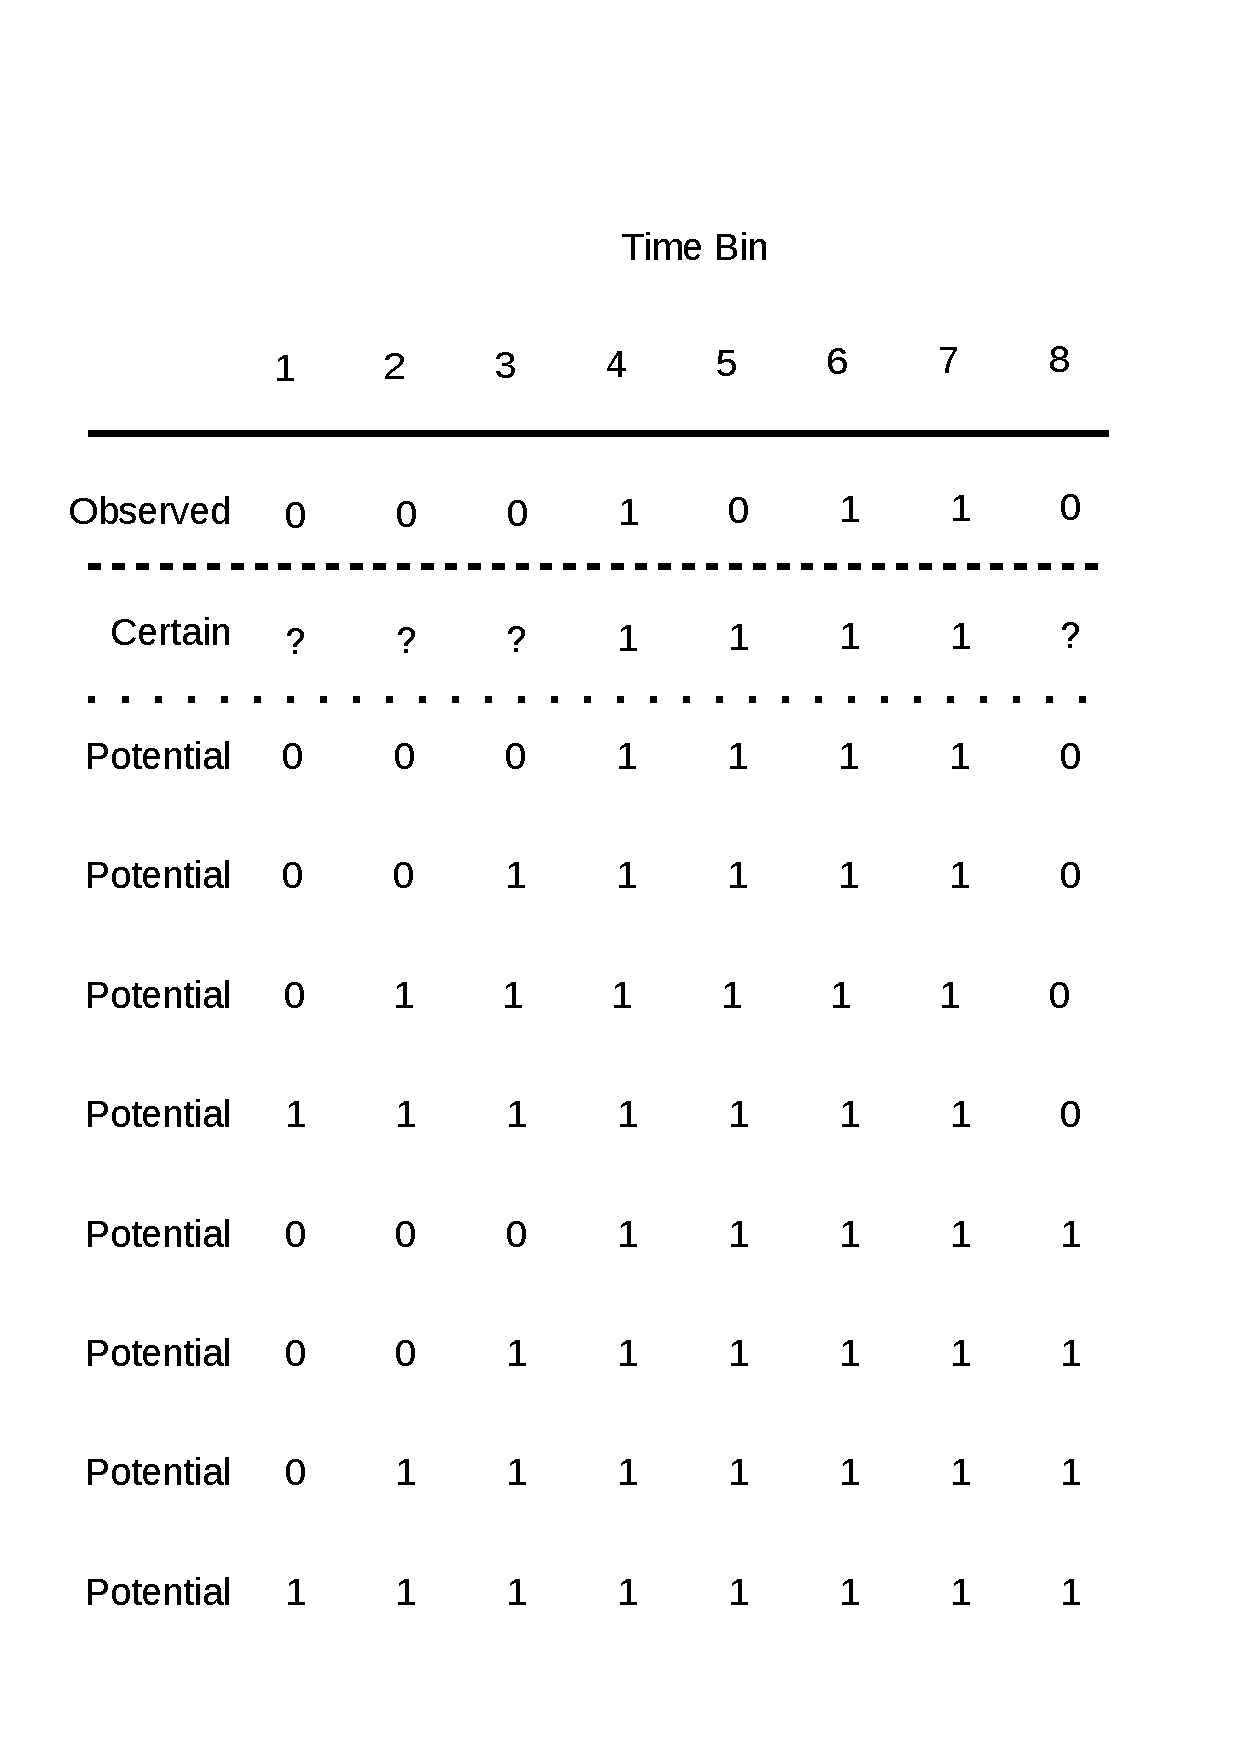
\includegraphics[height=0.4\textheight, width=\textwidth, keepaspectratio=true]{figure/margin}
  \caption[Conceptual figure of all possible occurrence histories for an observed species]{Conceptual figure of all possible occurrence histories for an observed species. The first row represents the observed presence/absence pattern for a single species at eight time points. The second row corresponds to the known aspects of the ``true'' occurrence history of that species. The remaining rows correspond to all possible occurrence histories that are consistent with the observed data. The process of parameter marginalization described in the text}
  \label{fig:margin_concept}
\end{figure}


% Stan
%   version 2.9.0
%   marginalize over latent discrete parameters
%     keeping in mind that species HAVE to range through
%     sum of the log probability for all possible configutations
%     along with the sampling probability given those combinations as well
%     see code for implementation? 
%       it is kind of an annoying amount of math to write up

The combined size of the dataset and large number of parameters in both models (Eqs. \ref{eq:pure_presence}, \ref{eq:birth_death}), specifically the total number of latent parameters that are the matrix \(z\), means that stochastic approximate posterior inference is computationally very slow even using NUTS based HMC implemented. Instead, an approximate Bayesian approach was used: variational inference. A recently developed automatic variational inference algorithm called ``automatic differention variational inference'' (ADVI) is implemented in Stan and was used here CITATION. ADVI assumes that the posterior is Gaussian but still yields a true Bayesian posterior; this assumption is similar to quadratic approximation of the likelihood function commonly used in maximum likelihood based inference CITATION. The principal limitation of assuming the joint posterior is Gaussian is that the true topology of the log-posterior isn't estimated; this is a particular burden for scale parameters which are bound to be positive (e.g. standard deviation).

Of additionaly concern for posterior inference is the partial identifiability of observation parameters \(p_{t = 1}\) and \(p_{t = T}\) \citep{Royle2008}. This issue means that the estimates of sampling probabilities at the ``edges'' of the time series cannot fully be estimated because there are no known ``gaps'' in species occurrence histories that are guarenteed to be filled. Instead, the values of the first and final columns of the ``true'' presence-absence matrix \(z\) for thos observations that do not already have presences in the observed presence-absence matrix \(y\) cannot be estimated \citep{Royle2008}. The hierarchical modeling approach used here helps mitigate this problem by pulling the values of \(p_{t = 1}\) and \(p_{t = T}\) towards the overall mean of \(p\) \citep{Gelman2013d}, and in fact this approach might be more analytically sound than the more ad-hob approaches that are occationally used to overcome this hurdle \citep{Royle2008}. Additionally, because \(p_{t = 1}\) and \(p_{t = T}\) are only partially identifiable, estimates of occurrence \(\theta\) and origination \(\phi\) at \(t = 1\) and estimates of \(\theta\), \(\phi\) and survival \(pi\) at \(t = T\) may suffer from similar edge effects. Again, the hierarchical modeling approach used here may help correct for this reality by drawing these estimates towards the overall means of those parameters.


After fitting both models (Eqs. \ref{eq:pure_presence}, \ref{eq:birth_death}) using ADVI, model adequacy and quality of fit was assessed using a simple posterior predictive check CITATION CITATION. Because all Bayesian models are inherently generative, simulations of new data sets is ``free'' CITATION. By simulating 100 theoretical data sets using the observed covariate information the congruence between predictions made by the model and the observed empirical data can be assessed. These datasets are simulated by starting with the observed states of the presence-absence matrix at \(t = 1\); from their, the time series roll forward as stochastic processes with covariate information given from the empirical observations. Importantly, this is fundamentally different from observing the posterior estimates of the ``true'' presence-absence matrix \(z\). The posterior predictive check used in this study is to compare the observed average number of observations per species to a distribution of simulated averages; if the empirically observed value sits in the middle of the distribution than the model can be considered adequate in reproducing the observed number of occurrences per species. 

The ADVI assumption of a purely Gaussian posterior limits the utility and accuracy of the posterior predictive checks because parameter estimates do not reflect the true posterior distribution and are instead just an approximation CITATIONS. Because of this, posterior predictive estimates are themselves only approximate checks of model adequacy. The posterior predictive check that is used in this study focuses on mean occurrence and not to any scale parameters that might be most affected by the ADVI assumptions.


Given parameter estimates, diversity and diversification rates are estimated through posterior predictive simulations. Given the observed presence-absence matrix \(y\), estimates of the true presence-absence matrix \(z\) can be simulated and the distribution of possible occurrence histories can be analyzed. This is conceptually similar to marginalization where the probability of each possible occurrence history is estimated (Fig. \ref{fig:margin_concept}). 

The posterior distribution of \(z\) gives the estimate of standing diversity \(N^{stand}_{t}\) for all time points as 
\begin{equation}
  N^{stand}_{t} = \sum_{i = 1}^{M} z_{i, t}.
  \label{eq:stand_est}
\end{equation}
Given estimates of \(N^{stand}\) for all time points, the estimated number of originations \(O_{t}\) are be estimated as 
\begin{equation}
  O_t = \sum_{i = 1}^{M} z_{i, t} = 1 | z_{i, t - 1} = 0
  \label{eq:orig_est}
\end{equation}
and number of extinctions \(E_{t}\) estimated as
\begin{equation}
  E_{t} = \sum_{i = 1}^{M} z_{i, t} = 0 | z_{i, t - 1} = 1.
  \label{eq:death_est}
\end{equation}
Per-captia growth \(D^{rate}\), origination \(O^{rate}\) and extinction \(E^{rate}\) rates are then calculated as
\begin{equation}
  \begin{aligned}
    O^{rate}_{t} &= \frac{O_t}{N^{stand}_{t - 1}} \\
    E^{rate}_{t} &= \frac{E_t}{N^{stand}_{t - 1}} \\
    D^{rate}_{t} &= O^{rate}_{t} - E^{rate}_{t}. \\
  \end{aligned}
  \label{eq:per_capita_est}
\end{equation}

% silly transforms using the poisson distribution aren't necessary if you just do the posterior simulations.
% discuss this in the discussion and not this section?


\end{document}
